\documentclass[11pt]{article}

% Font & ngôn ngữ tiếng Việt (pdfLaTeX)
\usepackage[utf8]{inputenc}
\usepackage[T5]{fontenc}


% Biblatex + biber
% \usepackage[backend=biber, style=numeric-comp, autolang=other]{biblatex}

%\addbibresource{references.bib} # tham khao

% Toán học & font Times
\usepackage{amsmath, amssymb, amsfonts, bm}

% Bảng biểu & căn lề
\usepackage{longtable}
\usepackage{array}
\usepackage{booktabs}

% Đồ họa & màu sắc
\usepackage{graphicx}
\usepackage{xcolor}
\usepackage{float}
\usepackage{subcaption}

% Liên kết & tham chiếu
\usepackage{hyperref}
\hypersetup{
    colorlinks=true,
    linkcolor=blue,
    urlcolor=red,
    pdftitle={Overleaf Example},
    pdfpagemode=FullScreen,
}

% Dấu tick và x
\usepackage{pifont}
\newcommand{\xmark}{\ding{55}}
\newcommand{\cmark}{\ding{51}}

% Tiêu đề tùy chỉnh
\usepackage{titling}
\setlength{\droptitle}{-10em}
\renewcommand{\maketitle}{
    \begin{center}
        \fontsize{18}{20}\selectfont\textbf{Avoid Training \& Predicting Data Conflict using Feast}\\[1em]
        \fontsize{14}{16}\selectfont Nhóm TimeSeries - GRID070\\[0.5em]
        \fontsize{14}{16}\selectfont Ngày 9 tháng 10 năm 2025
    \end{center}
    \vspace{1.5em}
}

% Format section (không đánh số)
\usepackage{titlesec}
\titleformat{\section}{\normalfont\Large\bfseries}{}{0em}{}

% Code block
\usepackage{listings}
\definecolor{backcolour}{rgb}{0.95,0.95,0.92}
\lstset{
    backgroundcolor=\color{backcolour},
    basicstyle=\ttfamily\footnotesize,
    breaklines=true,
    numbers=left,
    numberstyle=\tiny\color{gray},
    captionpos=b,
    language=python, % Đặt ngôn ngữ mặc định là bash cho lstlisting
    morekeywords={python, dvc, git, conda, mkdir, cd, pip, mklink, del}, % Thêm keywords
    commentstyle=\color{gray}, % Màu cho comment
    keywordstyle=\color{blue},
    stringstyle=\color{red}
}

% Hộp màu
\usepackage[many]{tcolorbox}
\definecolor{lightgreenbox}{rgb}{0.85,0.95,0.85}
\newtcolorbox{summarybox}{
    colback=lightgreenbox,
    colframe=green!50!black,
    boxsep=5pt, arc=4pt,
    boxrule=0.5pt,
    left=10pt, right=10pt,
    top=10pt, bottom=10pt,
}


% Layout trang
\setlength{\topmargin}{-0.7in}
\setlength{\textheight}{9.25in}
\setlength{\oddsidemargin}{0in}
\setlength{\textwidth}{6.8in}

%%%%%%%%%%%%%%%%%%%%%%%%%%%%%%%%%%%%%%%%%%%%%%%%%%%%%%%%%%%%%%%%%%%%%%%%%%%%%
\begin{document}

\maketitle

\begin{summarybox}
Nội dung về được chia thành 5 phần chính:
    \begin{itemize}
	\item \textbf{Revision: Data Versioning và ETL pipeline}
	\item \textbf{Overview: Giới thiệu vòng đời của 1 dự án Học Máy}
	\item \textbf{Feature Store và Feast là gì ?}
	\item \textbf{Case Study}
	\item \textbf{Final Revision: ôn lại mọi khái niệm trong bài cùng team Time Series}
    \end{itemize}
\end{summarybox}

% --- PHẦN 1 ---
\section{Intro: Từ ETL, Processing, Data Versoning đến Feature Store}

Hành trình của dữ liệu bắt đầu từ quy trình ETL (Extract, Transform, Load) để thu thập, chuẩn hóa dữ liệu thô từ nhiều nguồn đa dạng và làm sạch, biến đổi chúng rồi lưu trữ vào 1 trung tâm lưu trữ tập trung như Data Warehouse. \\
\begin{figure}[H]
    \centering
    \includegraphics[width=0.8\linewidth]{images/etl.png}
    \caption{ETL pipeline} 
\end{figure}

Tuy nhiên, trong thực tế để xử lý 1 lượng dữ liệu lớn là "động" được cập nhập liên tục (Streaming data như tin nhắn, đơn hàng shopee) và dữ liệu "tĩnh" ít thay đổi sau khi lưu (static như sách, thông tin cá nhân) tạo nhu cầu cho 1 phương pháp xử lý tinh vi hơn như Apache Spark cho phép ta xử lý đa luồng dữ liệu phức tạp cả tĩnh và động. Đồng thời hỗ trợ các tác vụ truy vấn (SparkSQL) và học máy (MLlib).
\begin{figure}[H]
    \centering
    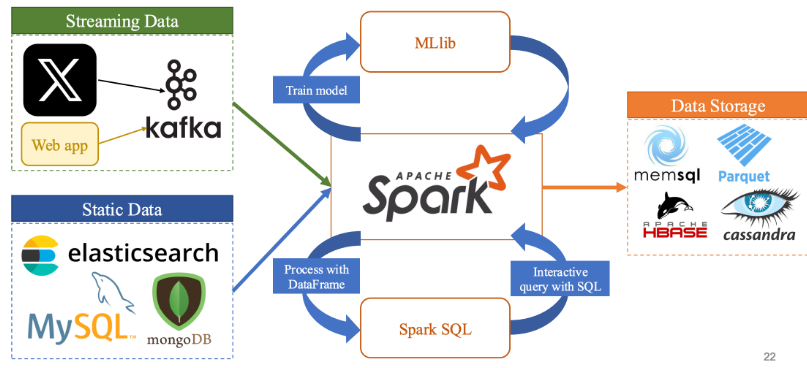
\includegraphics[width=0.8\linewidth]{images/proces.png}
    \caption{Process pipeline}
\end{figure}

Chính vì sự phát triển của các quy trình học máy đã tạo ra thách thức để quản lý mỗi phiên bản dữ liệu/mô hình bao gồm quản lý vô số artifacts như tệp tham số, phiên bản mô hình và bộ dữ liệu mới được tạo ra. Với Data Versioning, nó đảm bảo khả năng theo dõi, kiểm soát và tái thử nghiệm tương tự như cách Git quản lý mã nguồn. 
\begin{figure}[H]
    \centering
    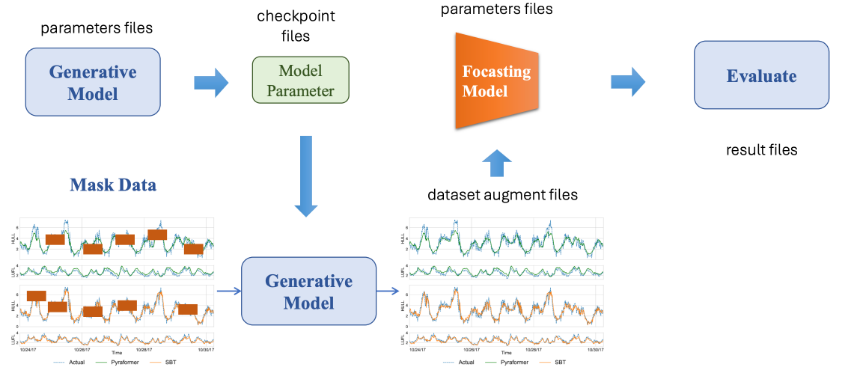
\includegraphics[width=0.8\linewidth]{images/dt_ver.png}
    \caption{Data versioning Pipeline}
\end{figure}

Cuối cùng sau khi đã lưu dữ liệu vào trung tâm lưu trữ data warehouse, xử lý dữ liệu lượng lớn cả tĩnh và động nhờ Apache Spark sau đó quản lý mỗi phiên bản dữ liệu/mô hình khi huấn luyện với data versioning, 1 câu hỏi được đặt ra là làm thế nào để kết hợp cả 3 quy trình để chuẩn hóa, lưu trữ rồi phục vụ các đặc trưng đã xử lý 1 cách nhất quán cho cả việc huấn luyện mô hình (training) và dự đoán (inference). Tất cả các bước trên đề hội tụ về một giải pháp trung tâm và hiệu quả: Feature Store. 


\section{ML/AI Project Lifecycle - Giới thiệu vòng đời của 1 dự án Học Máy}
\textbf{Data Engineering}
\textbf{Modeling}
\textbf{Deployment}
\textbf{Business analysis}
\textbf{AI Infrastructure - Cơ sở hạ tầng của 1 dự án AI}
\textbf{6 vai trò trong nhóm phát triển AI}

\section{Feature Store và Feast là gì ?}
Vấn đề chính trong ML Project life cycle.
Vấn đề Feature Store giải quyết
-> Các thành phần chính trong Feature Store pipeline
-> Lợi ích của Feature Store trong bố cảnh X. (liệt kê các lợi ích).

Feast thật sự là gì trong Feature ? (triết lý của Feast)
-> Feast Pipeline -> Các thành phần của Feast.

\section{Case Study}



\section{Final Revision: ôn lại mọi khái niệm trong bài cùng team Time Series}


%\printbibliography % Bỏ comment dòng này nếu bạn có tệp .bib

\end{document}

